% This text is a supplement of CINTA.
% May. 2018
% Author: Libin Wang
% SCNU
\documentclass{beamer}

%%%%%%%%%%%%%%%%%%%%%%%%%%%%%%%%%%%%%%%%%%%%%%%%%%%%%%%%%%%%%%%%%%%%%
\usepackage{xeCJK}
%\usepackage[CJKbookmarks]{hyperref}

%% Support Chinese with TeX Live fonts.
\setCJKmainfont[
  BoldFont=FandolHei-Regular.otf,
  ItalicFont=FandolKai-Regular.otf,
  BoldItalicFont=FandolKai-Regular.otf
]{FandolSong-Regular.otf}
\setCJKsansfont[AutoFakeBold, AutoFakeSlant]{FandolHei-Regular.otf}
\setCJKmonofont{FandolFang-Regular.otf}

%\setCJKmainfont[BoldFont=Microsoft YaHei,ItalicFont=YouYuan]{SimSun} %设置默认中文字体

\setmainfont{Times New Roman} % 设置默认英文衬线字体

\setCJKfamilyfont{ls}{FandolSong-Regular.otf} %定义字体
%%%%%%%%%%%%%%%%%%%%%%%%%%%%%%%%%%%%%%%%%%%%%%%%%%%%%%%%%%%%%%%%%%%%%

%\usepackage{beamerthemesplit} % new 
\usepackage{beamerthemeshadow}
\setbeamertemplate{headline}{}
\setbeamertemplate{navigation symbols}{}
\usepackage{amsmath, amsfonts, amssymb}

\usepackage[most]{tcolorbox}

%% Setup for Code
\usepackage{listings}
\lstset{language = Python,
	showstringspaces = false,
	columns = fullflexible,
	numbers = left,
	numberstyle = \tiny,
	frame = single}
%Can't work!
%\usepackage{minted}

%%\newproof{pf}{Proof} 
%\newtheorem{thm}{Theorem}[section]
%\newtheorem{fact}[theorem]{Fact}
\newtheorem{prop}[theorem]{Proposition}
\newtheorem{lem}[theorem]{Lemma}
\newtheorem{defn}[theorem]{Definition}
\newtheorem{cor}[theorem]{Corollary}
\newtheorem{rema}[theorem]{Remark}
\newtheorem{clam}[theorem]{Claim}
\newtheorem{exm}[theorem]{Example}

%\title{A Concrete Introduction to Number Theory and Algebra--Chapter 1- 2} 
\title{Mathematics for Computer Science -- 1} 
\author{王立斌} 
\institute{School of Computer Science, South China Normal University}
\date{\today} 

\begin{document}

\frame{\titlepage} 

\frame{\frametitle{Table of contents}\tableofcontents} 

%%%%%%%%%%%%%%%%%%%%% chapter.tex %%%%%%%%%%%%%%%%%%%%%%%%%%%%%%%%%
%
% Chapter 1. The integers
%
%%%%%%%%%%%%%%%%%%%%%%%% Springer-Verlag %%%%%%%%%%%%%%%%%%%%%%%%%%
%\motto{Use the template \emph{chapter.tex} to style the various elements of your chapter content.}
\section{Introduction.}
\frame{\frametitle{What is Mathematics for Computer Science -- 1?}
According to LLM17-MCS:
\begin{itemize}
\item Proof techniques -- 证明方法

\item Number Theory -- 初等数论

\item Abstract Algebra -- 抽象代数

\item Probability -- 概率论

\item Algorithms Analysis -- 算法分析
\end{itemize}

}

\frame{\frametitle{What is Mathematics for Computer Science -- 2?}
According to 《Concrete Mathematics》（GKP93--《具体数学》）：
\begin{itemize}

\item Number Theory -- 初等数论

\item Probability -- 概率论

\item Algorithms Analysis -- 算法分析相关的数学
\end{itemize}

\pause

\begin{alertblock}{本人浅见！}
《计算机科学中的数学》就是《离散数学》。
\end{alertblock}
}


\frame{\frametitle{Motivations of our course.}
从2024年起，《计算机科学中的数学》第一次出现在SCNU-CS，以下专题为本课程的主线:
\begin{itemize}
\item Number Theory -- 初等数论

\item Abstract Algebra -- 抽象代数

\item Algorithms -- 算法
\end{itemize}
\pause

\begin{alertblock}{Notice!}
强调，我们关注编程与算法，即所谓的"computational(计算性)"，且以上专题将融合在一起。
\end{alertblock}

}

\frame{\frametitle{参考书.}

\begin{itemize}
\item A Concrete Introduction to Number Theory and Algebra(CINTA，本课程教材)

\item Number Theory: A Friendly Introduction to Number Theory (FINT)

\item Abstract Algebra: Abstract Algebra: Theory and Applications (AATA)

\item Algorithms: Introduction to Algorithms (CLRS)
\end{itemize}
\pause

\begin{alertblock}{Wanted!}
Reading, thinking and programming.
\end{alertblock}

}

\frame{\frametitle{Remark.}
\begin{exampleblock}{本课程期望的目标.}
同学们可以建立起最基本、正常的数学学习思维，并多做练习.
\end{exampleblock}

\pause
\begin{exampleblock}{本课程一种重要的思路.}
Finding patterns. （寻找模式.）
\end{exampleblock}

}

% 20260302增补
\frame{\frametitle{AI时代的数学课特征与预警.}
\begin{exampleblock}{AI时代的数学课有什么特征.}
\begin{itemize}
	\item 更丰富的知识；更丰富的阅读资料；
	
	\item 更唾手可得的答案；
	 
\end{itemize}
\end{exampleblock}
\pause 
\begin{exampleblock}{AI时代的数学课需要警惕什么？}
\begin{itemize}
	\item 知识、资料过多，学习路径的选择更复杂；
	
	\item 容易得到答案，让本来就缺乏思考的大学生更难以抗拒惰性，“不思考”的状况进一步恶化；
	 
\end{itemize}
\end{exampleblock}
}

\section{Numbers in Computer Systems.}
\frame{\frametitle{Numbers.} 
	\begin{block}{Number systems}
 \[
 \mathbb{N} = \{0, 1, 2, \cdots \}
 \]
 \[
 \mathbb{Z} = \{0, \pm 1, \pm 2, \pm 3, \cdots \}
 \]
 \[\mathbb{Q}\]
 \[\mathbb{R}\]
 \end{block}
 
 \pause
 
 \begin{block}{问题.}
 计算机系统中的数学结构主要是什么？
 \end{block}
}

\frame{\frametitle{Warm-up-1.} 
	Simple Code:
	\begin{center}
		\lstinputlisting[language=C]{../codes/chap1-1.c}
	\end{center}

	\begin{block}{问题.}
		这段程序输出什么？
	\end{block}
}

\frame{\frametitle{Warm-up-2.} 
	Simple Code:
	\begin{center}
		\lstinputlisting[language=C]{../codes/chap1-2.c}
	\end{center}

	\begin{block}{问题.}
		这段程序输出什么？
	\end{block}
}

\frame{\frametitle{Warm-up-3.} 
\begin{exampleblock}{CSers的计算方法.}
\label{exm:binary}
请计算以下等式：
	\[1 + 2 + 2^2 + 2^3 + \cdots + 2^{10}\]
\end{exampleblock}	

\begin{block}{问题.}
	这道题的意义在哪里？
	\end{block}
}

\frame{\frametitle{Numbers in Computer Systems.} 
\begin{exampleblock}{Observations:}
	\begin{itemize}
		\item All computations in computers use fixed-size representations(定长计算).
		
		\item Addition（加法） is natural while multiplication（乘法） is not.
		
		\item Subtraction（减法） is the same as addition; the relation between multiplication and division（除法） is more complicated.
	\end{itemize}
\end{exampleblock}

\pause

\begin{alertblock}{注意!}
以下我们重点关注计算机系统中的加、减、乘、除.
\end{alertblock}
}

\frame{\frametitle{Simple rules for addition and multiplication.} 
\begin{exampleblock}{Well-known and useful rules of arithmetic:}
	\begin{itemize}
		\item The last bit of an even(odd) number is $0$($1$);
		
		\item To multiply(divide) an unsigned integer by $2$ is equivalent to shifting left(right) the number by $1$ bit.
	\end{itemize}
\end{exampleblock}
}

\frame{\frametitle{诡异的加法.} 

	\begin{center}
		\lstinputlisting[label = alg:add, title = 整数加法]{../codes/chap1-add.c}
	\end{center}

	\begin{block}{问题.}
		如何理解这个算法？
	\end{block}
}

\frame{\frametitle{理解加法.} 
要理解这个加法算法只需要正确回答出以下三个问题：

\begin{enumerate}
\item $a \wedge b$ 得到的是什么？

\item $(b \& a) << 1$ 得到的是什么？

\item 该算法为什么会终止？

\end{enumerate}
	
}

\section{Multiplication}

\frame{\frametitle{乘法的学习目标.} 
	\begin{block}{学习目标.}
		本节的主要内容：朴素乘法、简单乘法（递归版本与迭代版本）。建立算法分析的基本思路。
	\end{block}
}


\frame{\frametitle{Na\"{\i}ve Multiplication.} 
阅读并思考以下代码，理解它的计算方法。
	\begin{center}
		\lstinputlisting[language=Python]{../codes/chap1-3.py}
	\end{center}
\begin{block}{问题.}
	以上算法是否正确？效率如何？
\end{block}
}

\frame{\frametitle{Three key issues.} 
	In general, three key issues should be considered when we encounter a new algorithm.
	\begin{itemize}
		\item \textbf{Correctness(正确性)}. Does the algorithm correctly achieve the goal?
		
		\item \textbf{Efficiency(效率、复杂度)}.  How long does the algorithm take when it terminates?
		
		\item \textbf{Optimization(优化)}. Can we provide a better method?
	\end{itemize}
}

\frame{\frametitle{Rule of Multiplication.} 
为了得到计算$a * b $的优化算法，先思考以下递归的计算过程。
\begin{exampleblock}{Rule of Multiplication.}
	\begin{equation}  
	a \cdot b = 
	\left\{  
	\begin{array}{lr}  
	2(a\cdot \lfloor b/2 \rfloor ) &  \text{if $b$ is even;}\\  
	
	a +2(a\cdot \lfloor b/2 \rfloor) & \text{if $b$ is odd.} \\  
	
	\end{array}  
	\right.  
	\end{equation}
\end{exampleblock}
}

\frame{\frametitle{Simple multiplication的伪代码.} 
	\begin{center}
		\lstinputlisting[language=Python]{../codes/chap1-4.py}
	\end{center}
\begin{block}{问题.}
	以上算法是否正确？效率是否提高？
\end{block}

}

\frame{\frametitle{Simple multiplication的迭代版本.} 
如何得到一种迭代式的乘法算法？考虑以下表达式：
	\begin{exampleblock}{Intuition.}
		For two $n$-bits integers $a$ and $b$, view $b$ as a binary number in position notation(位置记数法).
		\begin{align*}
	      a \cdot b &= a \cdot (b_{n-1} 2^{n-1} + b_{n-2} 2^{n-2} + \cdots + b_1 2 + b_0)\\
	                &= b_{n-1}(a \cdot 2^{n-1}) + b_{n-2} (a \cdot 2^{n-2})+ \cdots + b_1(a\cdot 2) + b_0 a
		\end{align*}
	Observations:
	1. Every term in the last equation has $2^i a$, which means we must continue to do $a *= 2$
	
	2. The bit $b_i$ in every term plays as a flag, when $b_i=1$, we must have $res += a$;

	\end{exampleblock}
}

\frame{\frametitle{Simple multiplication的迭代版本.} 
位置计数法给我们的启发：
	\begin{exampleblock}{观察.}
		
	\begin{itemize}
		\item Every term in the last equation has $2^i a$, which means we must continue to do $a *= 2$
			\item The bit $b_i$ in every term plays as a flag, when $b_i=1$, we must have $res += a$;
	\end{itemize}

	\end{exampleblock}
}

\frame{\frametitle{Simple multiplication-计算实例.} 
	\begin{exampleblock}{Example.}
	To compute $3 \times 10$. \pause
	
	$10$'s binary string is $1010$. \pause
	
	Repeatedly multiply $3$ by $2^i$ and get: 3, 6, 12, 24. \pause
	
	Choose the right terms to add, they are 6 and 24. \pause
	
	Return the result which is 30.

	\end{exampleblock}
}

\frame{\frametitle{Simple multiplication.} 
	\begin{exampleblock}{Analysis}
		\begin{itemize}
			\item Correctness. Obviously.
			
			\item Efficiency. $\mathcal O (n^2)$ bit operations. Why?
			
			\item Optimization. To be or not to be optimized? Why?
		\end{itemize}
	\end{exampleblock}

\begin{block}{Notice!}
The multiplication is implemented \emph{without} using multiplication !
\end{block}
}

\frame{\frametitle{Remarks.} 

\begin{block}{思考.}
请不要把这里的“加、减、乘、除”仅仅视为计算机系统中需要实现的计算方法，而应该把它们理解为某种“模式”、某种“思维方式”。请在后续课程中不断体会。
\end{block}
}

\frame[shrink=15]{\frametitle{练习题.} 
对比以下两种数列求积算法，说明并验证它们的效率。

	\begin{center}
		\lstinputlisting[language=Python]{../codes/product1.py}
	\end{center}
	
		\begin{center}
			\lstinputlisting[language=Python]{../codes/product2.py}
		\end{center}
}

%%%
\section{Division.}

\frame{\frametitle{除法.} 
	\begin{block}{本节学习目标.}
		本节的主要内容：除法算法、良序公理、除法算法的证明。
	\end{block}
}
\frame{\frametitle{ Division Algorithm.}

\begin{theorem} (Division Algorithm)
	Given integers  $a$ and $b$, with $b > 0$, there exist unique integers $q$ and $r$, called \emph{quotient}（商） and \emph{remainder}（余数） respectively, such that 
	%
		\[
		a = qb + r
		\]
	%
	where $0 \leq r < b$.
\end{theorem}

\begin{block}{Remark.}
	除法算法并不仅仅是算法或定理。
\end{block}
}

\frame{\frametitle{Geometric interpretation of division.} 
	
	\begin{figure}
		\begin{center}
		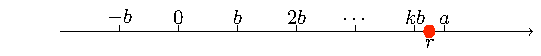
\includegraphics[scale=1]{../figures/mod.pdf} 
		\caption{Geometric interpretation of division.}
		\end{center}
		
		\label{fig:1}       % Give a unique label
	\end{figure}
\begin{block}{Remark.}
	除法算法的几何解释能在后续帮助我们设计算法，请留意。
\end{block}
}

\frame{\frametitle{Axiom.} 
在证明除法算法之前，先解释一种常用公理。
\begin{exampleblock}{Principle of Well-Ordering(良序原则).}
	Every nonempty subset of natural numbers  contain a least element.
\end{exampleblock}	
}

\frame{\frametitle{Proof of division theorem.} 
The proof contains two parts: existence(存在性) and uniqueness(唯一性).
	\begin{proof}
		\begin{itemize}
			\item \textbf{Existence of $q$ and $r$.} 
		证明存在性使用什么方法？\pause
		
		构造法：Given $a$ and $b$, construct a set
		\[
		S = \{ a - bk : k \in \mathbb{Z} \; \text{and}\; (a - bk) \geq 0 \}.
		\]
		
		\end{itemize}
		
	\end{proof}
}

\frame{\frametitle{Proof of division theorem（Continue）.} 
	
	\begin{proof}
		
		\begin{itemize}
		\item 
		It is easy to show that $S$ is nonempty. By the \textbf{Principle of Well-Ordering}, there is a smallest member $r \in S$, and $r = a - qb$. Therefore, $a = qb + r$, $r \geq 0$. To show $r < b$ is left as an exercise.

		\item \textbf{Uniqueness of $q$ and $r$.} This is an exercise. [提示：证明唯一性使用什么方法？反证法！]
		\end{itemize}
		
	\end{proof}
}

\frame{\frametitle{Na\"{\i}ve Division.} 
算法的实现：
\begin{center}
	\lstinputlisting[language=Python]{../codes/chap1-5.py}
\end{center}

\begin{block}{问题.}
	算法是否正确？效率如何？能否优化？
\end{block}
}

\frame{\frametitle{ Simple Division.} 
\begin{center}
	\lstinputlisting[language=Python]{../codes/chap1-6.py}
\end{center}

}

\frame{\frametitle{ Simple Division-思考.} 
\begin{block}{问题.}
	算法是否正确？效率如何？是否对朴素除法的优化？为什么？
\end{block}
}

\frame{\frametitle{ Important remark.}
\begin{block}{重要提示.}
Multiplication can be implemented using only addition and shifts, while division can be implemented using only subtraction and shifts. More importantly, the point is not merely implementation, but a way of thinking that will reappear throughout the course.
\end{block}
} 
\section{The Euclidean Algorithm}

\frame{\frametitle{欧几里得算法.} 
以下我们转入一个新的主题：欧几里得算法。先介绍一些定义与概念。	
    \begin{itemize}
		\item \textbf{Divisibility. }Let $a$ and $b$ be integers, $a$ is said to be  \emph{divisible}  by $b$ when $a = qb$ for some integer $q$, we write $b \mid a$. 
		
		\item \textbf{Common divisor. }An integer $d$ is called a common divisor of $a$ and $b$ if $d \mid a$ and $d \mid b$. 
		
		\item \textbf{Greatest common divisor.} An integer $d$ is the greatest common divisor($\gcd$) of $a$ and $b$, if $d$ is a common divisor of $a$ and $b$, and for any other common divisor of $a$ and $b$, say $d'$, then $d' \mid d$. 
		
			\item \textbf{Relatively prime.} If $\gcd(a, b) = 1$, we say that $a$ and $b$ are relatively prime. 
	\end{itemize}
}

\label{sec:gcd}
% Always give a unique label
\frame{\frametitle{The Euclidean Algorithm.} 
   \begin{exampleblock}{Euclidean algorithm($\gcd$ algorithm).}
	Given two positive integers $a$ and $b$ with $a \geq b$:
	\[
	\gcd(a, b) = \gcd(b, a  \bmod{b})
	\]
	where $a \bmod{b}$ means to divide $a$ by $b$ to get the remainder $r$.
  \end{exampleblock}
}

\frame{\frametitle{The Euclidean Algorithm.} 
一个计算实例。
	\begin{exm}
		\label{exm:gcd}
		Given $a = 12345$ and $b = 678$, 
		 \begin{align*}
         \gcd(12345, 678)
         &= \gcd(678, 141) \\
         &= \gcd(141, 114) \\
         &= \gcd(114, 27) \\
         &= \gcd(27, 6) \\
         &= \gcd(6, 3) \\
         &= \gcd(3, 0)
         \end{align*}
  
		Hence, $\gcd(12345, 678) = 3$.
	\end{exm}
}

\frame{\frametitle{The Euclidean Algorithm.} 
$\gcd$算法的递归实现如下：
\begin{center}
	\lstinputlisting[language=Python]{../codes/chap1-7.py}
\end{center}
}


\frame{\frametitle{Correctness of The Euclidean Algorithm.} 
	\noindent\textbf{Correctness.} It is enough to show a slightly simpler rule:
	\[
		\gcd(a, b) = \gcd(a - b,  b).
	\]
	From this rule, we can repeatedly subtract $b$ from $a$ (recall the Na\"{\i}ve division algorithm) and derive the final rule as follows:
	\begin{align*}
		\gcd(a, b)
		&= \gcd(a - b,  b) \\
		&= \gcd((a - b) - b, b) \\
		&= \cdots \\
		&= \gcd(a \mod  b,  b).
	\end{align*}
}


\frame{\frametitle{Correctness of The Euclidean Algorithm.} 
	
	To show $\gcd(a, b) = \gcd(a - b,  b)$, we have two directions to prove. 
	\begin{itemize}
	\item any integer that divides both $a$ and $b$ must also divides $a - b$, thus $\gcd(a, b) \leq \gcd(a - b, b)$. 
	
	\item any integer that divdes both $a-b$ and $b$ must also divide $a$ and $b$, thus $\gcd(a-b, b) \leq \gcd(a, b)$.
	\end{itemize}
}

\frame{\frametitle{Efficiency of The Euclidean Algorithm.} 
\noindent\textbf{Efficiency.}
	To understand that the $\gcd$ algorithm is quite fast, we should be aware of the fact that $a \mod b$ is a substantial reduction. It is easy to check:
	\begin{lem}
		If $a \geq b$, then $(a \bmod b ) < a/2$. 
	\end{lem}
	Hence, after two consecutive rounds, both $a$ and $b$ are at least halved in value, which means that the algorithm will terminate after $\mathcal O(\log a)$ recursive calls.\\
}

\frame{\frametitle{Optimization of The Euclidean Algorithm.} 
	Can we do better? The \textit{binary gcd algorithm}, also known as Stein's algorithm, has the same function as the $\gcd$ algorithm. This algorithm avoids complex operations, such as division and multiplication; instead, it relies only on subtraction, and more efficient bit right shift and bit left shift operations. The analysis of binary gcd algorithm is an exercise.
}


\section{The Extended Euclidean Algorithm}
\label{sec:egcd}
\frame{\frametitle{B\'{e}zout's Theorem.} 
	\begin{theorem}(B\'{e}zout)
		\label{thm:bezout}
		Let $a$ and $b$ be nonzero integers. Then there exist integers $r$ and $s$  such that 
			\[
			\gcd(a,b) = ar + bs
			\]
		Furthermore, the greatest common divisor of $a$ and $b$ is unique.
	\end{theorem}\pause
	
}

\frame{\frametitle{Proof of B\'{e}zout's Theorem-- 提示1.} 

	\begin{proof}
	构造集合
		 \[S = \{ am + bn : m,n  \in \mathbb{Z} \; \text{且}\; am + bn > 0 \}.\]
	显然，集合$S$非空，根据良序原则，取其中最小值$d = ar + bs$。然后证明两个属性：$d$是$a$和$b$的公因子（提示：除法算法！）；
	如果存在$a$和$b$的公因子$d'$，则$d' \mid d$。这样就证明了$d= \gcd(a,b)$。
	\end{proof}
}

\frame{\frametitle{Proof of B\'{e}zout's Theorem-- 提示2.} 

	\begin{proof}
	证明$d$整除$a$。根据除法算法，
	记$a = d q + r'$，$0 \leq r' < d$。证明$r' = 0$。
    如果$r' > 0$，则有：
 		\begin{align*}
       r' &= a - d q \\
          &= a - (ar + bs) q \\
          &= a(1 - qr) + b(-qs)
      		\end{align*}
	所以，$r'$也落在集合$S$中，但是，这与$d$是集合$S$中最小元素矛盾。
	因此，$r'$只能是$0$。
	同理，可证$d$整除$b$。请读者完成余下细节，留作练习。
	\end{proof}
}

\frame{\frametitle{B\'{e}zout's Theorem的应用.} 
 B\'{e}zout定理的证明还显示这样一个重要的事实：
	\begin{center}
	\begin{tcolorbox}[colback=green!5!white, colframe=red!75!black,width = 10cm]
$\gcd(a,b)$等于$a$和$b$所有线性组合值的最小值。
	\end{tcolorbox}
	\end{center}
记住这个事实，它可经常帮助我们解题。比如，我们立即可得以下推论。

\begin{corollary}
整数$a$和$b$互素当且仅当存在整数$r$和$s$使得$ar + bs = 1$。
\end{corollary}
}

\frame{\frametitle{B\'{e}zout's Theorem的应用.} 
 \begin{theorem}
 %	\label{thm:euclid1}
 	设$a, b \in \mathbb{Z}$，$p$为素数。如果$p \mid ab$，则$p \mid a$或$p \mid b$。
 \end{theorem}
 \pause
 \begin{proof}
 假设$p \nmid a$，证明$p \mid b$。因为$p \nmid a$且$p$是素数，则$\gcd(a, p) = 1$，即存在$r,s \in \mathbb{Z}$使得$ar + ps = 1$。因此，
 \[
 b = b(ar + ps) = abr + pbs.
 \]
 既然$p \mid ab$，那么$p$同时整除$abr$和$pbs$，则$p$必然整除$b$. 
 \end{proof}
}

\frame{\frametitle{B\'{e}zout's Theorem的应用.} 
 \begin{corollary}
 %\label{cor:euclid1}
 	设$a, b , n\in \mathbb{Z}$，$n>0$。如果$n \mid ab$且$\gcd(a, n)=1$，则$n \mid b$.
 \end{corollary}
 
 \begin{proof}
 使用以上类似的方法，易得，留作练习。
 \end{proof}
}


\frame{\frametitle{The Extended Euclidean Algorithm.} 
		\begin{exampleblock}{The extended Euclidean algorithm. }
		The \textit{extended Euclidean algorithm}(egcd-algorithm) is a simple extension of the Euclidean algorithm. Given two nonzero integers $a$ and $b$,  it  efficiently computes the \textit{B\'{e}zout coefficients} $r$ and $s$, and plays an important role in modular arithmetic.
	\end{exampleblock}
	
}

\frame{\frametitle{The Extended Euclidean Algorithm.} 
	\begin{exm}
		\label{exm:egcd1}
		Given $a = 19$, $b = 13$, to find $r$ and $s$, such that $ar + bs = \gcd(19, 13)$. 
		\begin{align}
		a\cdot 1 + b\cdot 0 &= 19\\
		a\cdot 0 + b\cdot 1 &= 13
		\end{align}
		\begin{align}
		a \cdot 1 + b\cdot (-1) &= 6
		\end{align}
		\begin{align}
		a \cdot (-2) + b\cdot 3 &= 1
		\end{align}
		Finally, we have $r = -2$, $s = 3$ and $d = 1$, which is the answer.
	\end{exm}
}

\frame{\frametitle{The Extended Euclidean Algorithm.} 
	\begin{exampleblock}{Recapitulate the process. }
	\begin{itemize}
		\item Write out two obviously true linear equations.
		
		\item Repeatedly subtract some integer multiple of one equation from the other, until the right-hand side of one equation achieves $\gcd(a,b)$.
	\end{itemize}
   \end{exampleblock}
}

\frame{\frametitle{The Extended Euclidean Algorithm.} 
	\begin{exampleblock}{Two Observations.}
	
	At least two facts should be noticed
	\begin{itemize}
	
	\item The right-hand sides of these equations undergo the same iterations as in the Euclidean algorithm.
	
	\item The $a$ and $b$ are just place holders, they are not involved in the computation, we can safely get rid of them in the equations.
	
	\end{itemize}
   \end{exampleblock}
}

\frame{\frametitle{The Extended Euclidean Algorithm.} 
	\begin{exampleblock}{例子}
		Given $a = 13$, $b = 9$, to find $r$ and $s$, such that $ar + bs = \gcd(13, 9)$. We write out a matrix:
		\begin{align*}
		\begin{pmatrix} 
		1 && 0 && 13\\
		0 && 1 && 9
		\end{pmatrix}
		\end{align*}
		If we subtract row 2 from row 1, we get a new matrix:
		\begin{align*}
		\begin{pmatrix} 
		0 && 1 && 9\\
		1 && -1 && 4
		\end{pmatrix}
		\end{align*}
	\end{exampleblock}
}
\frame{\frametitle{The Extended Euclidean Algorithm.} 
	\begin{exampleblock}{例子-续}
		Then we subtract 2 multiple of row 2 from row 1, we get:
		\begin{align*}
		\begin{pmatrix} 
		1 && -1 && 4\\
		-2 && 3 && 1
		\end{pmatrix}
		\end{align*}
		Finally, we have $r = -2$, $s = 3$ and $d = 1$, which is the answer. 
	\end{exampleblock}
}

\frame{\frametitle{The Extended Euclidean Algorithm.} 
	%%% From a perspective of matrix,  
	From the perspective of matrix,  the process starts with a matrix
	\begin{align*}
	M &= 
	\begin{pmatrix} 
	1 && 0 && a\\
	0 && 1 && b
	\end{pmatrix}
	\end{align*}
	which satisfies
	\begin{align*}
	M  
	\begin{pmatrix} 
	a\\
	b\\
	-1
	\end{pmatrix}
	=
	\begin{pmatrix} 
	0\\
	0
	\end{pmatrix}
	\end{align*}
	By repeatedly subtracting a multiple of one row of $M$ from the other row or exchanging the two rows, finally we obtain a matrix $M'$
	\begin{align*}
	M' &= 
	\begin{pmatrix} 
	r && s && d\\
	R && S && 0
	\end{pmatrix}
	\end{align*}

}

\frame{\frametitle{The Extended Euclidean Algorithm.} 
	%%% From a perspective of matrix,  
	\begin{align*}
	M' &= 
	\begin{pmatrix} 
	r && s && d\\
	R && S && 0
	\end{pmatrix}
	\end{align*}
    satisfies
	\begin{align*}
	M'  
	\begin{pmatrix} 
	a\\
	b\\
	-1
	\end{pmatrix}
	=
	\begin{pmatrix} 
	0\\
	0
	\end{pmatrix}
	\end{align*}
	That means $ar + bs = d$.
}

\frame{\frametitle{课堂练习.} 
	\begin{exampleblock}{课堂练习.}
		Given $a = 252$, $b = 198$, to find $r$, $s$ and $d = \gcd(a, b)$, such that $ar + bs = d$.
	\end{exampleblock} 
	%%% 4, -5, 18
}

\frame{\frametitle{The  Extended Euclidean Algorithm.} 
	The extended Euclidean algorithm is essentially the process of computing B\'{e}zout coefficients we described above.
	\begin{center}
		\lstinputlisting[language=Python]{../codes/chap1-9.py}
	\end{center}
}

\frame{\frametitle{Analysis of The  Extended Euclidean Algorithm.} 
	\begin{itemize}
		\item Correctness: it is easy.
		
		\item Efficiency: it is trivial.
		
		\item Optimization: binary-egcd.
	\end{itemize}
}

\frame{\frametitle{Concluding Remarks.}
	 	\begin{itemize}
	    \item The content is easy, but is not trivial.
	 	
	 	\item Algorithms should be focused by CSers.
	 	
	 	\item Useful tools should be mastered.
	   \end{itemize}
}

\frame{\frametitle{Happy ending.}
	\begin{itemize}
	\item Any questions?
	
	\item Feedback is welcome: lbwang@gmail.com. 
	
	\item Thanks!
\end{itemize}
}

\end{document}
